% Options for packages loaded elsewhere
\PassOptionsToPackage{unicode}{hyperref}
\PassOptionsToPackage{hyphens}{url}
\PassOptionsToPackage{dvipsnames,svgnames,x11names}{xcolor}
%
\documentclass[
  article]{jss}

\usepackage{amsmath,amssymb}
\usepackage{iftex}
\ifPDFTeX
  \usepackage[T1]{fontenc}
  \usepackage[utf8]{inputenc}
  \usepackage{textcomp} % provide euro and other symbols
\else % if luatex or xetex
  \usepackage{unicode-math}
  \defaultfontfeatures{Scale=MatchLowercase}
  \defaultfontfeatures[\rmfamily]{Ligatures=TeX,Scale=1}
\fi
\usepackage{lmodern}
\ifPDFTeX\else  
    % xetex/luatex font selection
\fi
% Use upquote if available, for straight quotes in verbatim environments
\IfFileExists{upquote.sty}{\usepackage{upquote}}{}
\IfFileExists{microtype.sty}{% use microtype if available
  \usepackage[]{microtype}
  \UseMicrotypeSet[protrusion]{basicmath} % disable protrusion for tt fonts
}{}
\makeatletter
\@ifundefined{KOMAClassName}{% if non-KOMA class
  \IfFileExists{parskip.sty}{%
    \usepackage{parskip}
  }{% else
    \setlength{\parindent}{0pt}
    \setlength{\parskip}{6pt plus 2pt minus 1pt}}
}{% if KOMA class
  \KOMAoptions{parskip=half}}
\makeatother
\usepackage{xcolor}
\setlength{\emergencystretch}{3em} % prevent overfull lines
\setcounter{secnumdepth}{-\maxdimen} % remove section numbering
% Make \paragraph and \subparagraph free-standing
\ifx\paragraph\undefined\else
  \let\oldparagraph\paragraph
  \renewcommand{\paragraph}[1]{\oldparagraph{#1}\mbox{}}
\fi
\ifx\subparagraph\undefined\else
  \let\oldsubparagraph\subparagraph
  \renewcommand{\subparagraph}[1]{\oldsubparagraph{#1}\mbox{}}
\fi


\providecommand{\tightlist}{%
  \setlength{\itemsep}{0pt}\setlength{\parskip}{0pt}}\usepackage{longtable,booktabs,array}
\usepackage{calc} % for calculating minipage widths
% Correct order of tables after \paragraph or \subparagraph
\usepackage{etoolbox}
\makeatletter
\patchcmd\longtable{\par}{\if@noskipsec\mbox{}\fi\par}{}{}
\makeatother
% Allow footnotes in longtable head/foot
\IfFileExists{footnotehyper.sty}{\usepackage{footnotehyper}}{\usepackage{footnote}}
\makesavenoteenv{longtable}
\usepackage{graphicx}
\makeatletter
\def\maxwidth{\ifdim\Gin@nat@width>\linewidth\linewidth\else\Gin@nat@width\fi}
\def\maxheight{\ifdim\Gin@nat@height>\textheight\textheight\else\Gin@nat@height\fi}
\makeatother
% Scale images if necessary, so that they will not overflow the page
% margins by default, and it is still possible to overwrite the defaults
% using explicit options in \includegraphics[width, height, ...]{}
\setkeys{Gin}{width=\maxwidth,height=\maxheight,keepaspectratio}
% Set default figure placement to htbp
\makeatletter
\def\fps@figure{htbp}
\makeatother

\usepackage{orcidlink,thumbpdf,lmodern}

\newcommand{\class}[1]{`\code{#1}'}
\newcommand{\fct}[1]{\code{#1()}}
\makeatletter
\makeatother
\makeatletter
\makeatother
\makeatletter
\@ifpackageloaded{caption}{}{\usepackage{caption}}
\AtBeginDocument{%
\ifdefined\contentsname
  \renewcommand*\contentsname{Table of contents}
\else
  \newcommand\contentsname{Table of contents}
\fi
\ifdefined\listfigurename
  \renewcommand*\listfigurename{List of Figures}
\else
  \newcommand\listfigurename{List of Figures}
\fi
\ifdefined\listtablename
  \renewcommand*\listtablename{List of Tables}
\else
  \newcommand\listtablename{List of Tables}
\fi
\ifdefined\figurename
  \renewcommand*\figurename{Figure}
\else
  \newcommand\figurename{Figure}
\fi
\ifdefined\tablename
  \renewcommand*\tablename{Table}
\else
  \newcommand\tablename{Table}
\fi
}
\@ifpackageloaded{float}{}{\usepackage{float}}
\floatstyle{ruled}
\@ifundefined{c@chapter}{\newfloat{codelisting}{h}{lop}}{\newfloat{codelisting}{h}{lop}[chapter]}
\floatname{codelisting}{Listing}
\newcommand*\listoflistings{\listof{codelisting}{List of Listings}}
\makeatother
\makeatletter
\@ifpackageloaded{caption}{}{\usepackage{caption}}
\@ifpackageloaded{subcaption}{}{\usepackage{subcaption}}
\makeatother
\makeatletter
\makeatother
\ifLuaTeX
  \usepackage{selnolig}  % disable illegal ligatures
\fi
\IfFileExists{bookmark.sty}{\usepackage{bookmark}}{\usepackage{hyperref}}
\IfFileExists{xurl.sty}{\usepackage{xurl}}{} % add URL line breaks if available
\urlstyle{same} % disable monospaced font for URLs
\hypersetup{
  pdftitle={Interplot: Plot the Effects of Variables in Interaction Terms},
  pdfauthor={Frederick Solt; Yue Hu},
  pdfkeywords={interplot, interaction effect, ordinary linear regression
models, generalized linear models, multilevel regressions, ggplot},
  colorlinks=true,
  linkcolor={blue},
  filecolor={Maroon},
  citecolor={Blue},
  urlcolor={Blue},
  pdfcreator={LaTeX via pandoc}}

%% -- Article metainformation (author, title, ...) -----------------------------

%% Author information
\author{Frederick Solt\\University of Iowa \And Yue Hu\\Tsinghua
University}
\Plainauthor{Frederick Solt, Yue Hu} %% comma-separated

\title{Interplot: Plot the Effects of Variables in Interaction Terms}
\Plaintitle{Interplot: Plot the Effects of Variables in Interaction
Terms} %% without formatting

%% an abstract and keywords
\Abstract{The interplot package provides a flexible and convenient way
to visualize conditional coefficients of variables in multiplicative
interaction terms. Comparing to established alternatives such as
effects::plot and sjplot::sjp.int, interplot provides a more
user-friendly way to quickly produce plots that are easy to interpret.}

%% at least one keyword must be supplied
\Keywords{interplot, interaction effect, ordinary linear regression
models, generalized linear models, multilevel regressions, ggplot}
\Plainkeywords{interplot, interaction effect, ordinary linear regression
models, generalized linear models, multilevel regressions, ggplot}

%% publication information
%% NOTE: Typically, this can be left commented and will be filled out by the technical editor
%% \Volume{50}
%% \Issue{9}
%% \Month{June}
%% \Year{2012}
%% \Submitdate{2012-06-04}
%% \Acceptdate{2012-06-04}
%% \setcounter{page}{1}
%% \Pages{1--xx}

%% The address of (at least) one author should be given
%% in the following format:
\Address{
Frederick Solt\\
E-mail: \email{frederick-solt@uiowa.edu}\\
\\~
Yue Hu\\
E-mail: \email{yuehu@tsinghua.edu.cn}\\
\\~

}

\begin{document}
\maketitle
\hypertarget{sec-introduction-apowerful-tool-to-test-conditional-effects}{%
\section{Introduction: A powerful tool to test conditional
effects}\label{sec-introduction-apowerful-tool-to-test-conditional-effects}}

Interaction is a powerful tool to test conditional effects of one
variable on the contribution of another variable to the dependent
variable and has been extensively applied in the empirical research of
social science since the 1970s\citep{Wright1976}. Unfortunately, the
nonlinear nature determines that the statistical estimate of an
interactive effect cannot be interpreted as straightforward as the
coefficient of a regular regression parameter. Let's use a simple
example to illustrate this point: The following model use an interaction
term to test the conditional effect of Z on X's contribution (or the
conditional effect of X on Z's contribution) to the variance of Y.

\[
Y = \beta_0 + \beta_1X + \beta_2Z + \beta_3X\times Z + \varepsilon.
\]

The contribution of X on Y is typically represented by the marginal
effect: \[
\frac{\partial Y}{\partial X} = \beta_1 + \beta_3Z.
\] The standard error of this estimate is thus: \[
\hat{\sigma}_{\frac{\partial Y}{\partial X}} = \sqrt{var(\hat{\beta_1}) + Z^2var(\hat{\beta_3}) + 2Zcov(\hat{\beta_1}, \hat{\beta_3})}.
\] As \citep{BramborClarkGolder2006}{[}p.70{]} indicates, the above
equation suggests that its perfectly possible for the contribution of X
on Y to be statistically significant for certain values of Z ``even if
all of the model parameters are insignificant.'' In other words, one
cannot infer whether X has a meaningful conditional effect on Y simply
from the magnitude and significance of either β1 or β3 (Ibid., 74).
Instead, the conditional effect should be examined based on the marginal
effect at every observed value of Z
\citep{BerryGolderMilton2012, BramborClarkGolder2006, Braumoeller2004}.

Furthermore, scholars have noticed that the point estimations of some
interaction models, especially those depending on link functions (e.g.,
logit and probit) may not be as reliable as the estimates of the
confidence intervals \citep{BerryDeMerittEsarey2016}. Therefore, it is
even more important to accurately present and examine the boundaries
established by the confidence intervals than the point estimates in the
test of conditional effect. \citep{BerryGolderMilton2012} also pointed
out that the substantive significance of the conditional effect highly
relates to the distribution of the conditioning variable (viz., Z in the
above example). They thus recommend researchers to present the frequency
distribution of the conditioning variable together with the marginal
effects (especially when the effect trend goes across the zero point).

More recently, \citep{EsareySumner2018}uncovered that the estimation of
the marginal effects suggested by \citep{BramborClarkGolder2006} might
cause a ``multiple comparison problem'' and result over- or
underconfidence of the confidential intervals. They thus recommended to
adjust the CIs with a critical t-statistics following the Benjamini1995
procedure.

The \texttt{interplot} package provides a convenient way to operate and
visualize above points with one or a series of plots produced by a
single function. The function visualizes the changes in the coefficient
of one variable in a two-way interaction term conditional on the value
of the other included variable. The plot also includes simulated 95\%
confidential intervals of these coefficients. In the current version,
the function works with ordinary linear regression models, generalized
linear models (e.g., logit, probit, ordered logit, etc.), and multilevel
(mixed-effects) regressions, all with complete or multiply imputed data.

Comparing to established alternatives such as \texttt{effects::plot} and
\texttt{sjplot::sjp.int}, \texttt{interplot} provides a more
user-friendly way to quickly produce plots that are easy to interpret.
\texttt{interplot} plots the changes in the \emph{conditional
coefficient} of one variable in the interaction, rather than changes in
the dependent variable itself as in the aforementioned functions. This
approach avoids displaying interaction effects across multiple panels or
multiple lines in favor of a single plot containing all the relevant
information. Moreover, by outputting \texttt{ggplot} objects,
\texttt{interplot} allows users to easily further customize their
graphs.

\hypertarget{sec-installation}{%
\section{Installation}\label{sec-installation}}

To install:

\begin{itemize}
\item
  the latest released version: \texttt{install.packages("interplot")}.
\item
  the latest developing version:
  \texttt{devtools::install\_github("sammo3182/interplot")}.
\end{itemize}

\hypertarget{sec-basic-use}{%
\section{Basic Use}\label{sec-basic-use}}

\hypertarget{sec-run-a-model}{%
\subsection{Run a Model}\label{sec-run-a-model}}

This example is based on the \texttt{mtcars} dataset, which is drawn
from the 1974 volume of the US magazine \emph{Motor Trend}. The
dependent variable is mileage in miles per (US) gallon (\texttt{mpg}),
and the independent variables are the number of engine cylinders
(\texttt{cyl}) and automobile weight in thousands of pounds
(\texttt{wt}).

\begin{verbatim}
data(mtcars)  #load the data
\end{verbatim}

Suppose we are interested in how automobile weight affects the
relationship between of the number of engine cylinders on mileage and
how the number of cylinders affects the relationship between the car's
weight and its mileage. Such conditional effects are modeled using a
two-way multiplicative interaction term:

\begin{verbatim}
m_cyl <- lm(mpg ~ wt * cyl, data = mtcars)
summary(m_cyl)
\end{verbatim}

\begin{verbatim}

Call:
lm(formula = mpg ~ wt * cyl, data = mtcars)

Residuals:
    Min      1Q  Median      3Q     Max 
-4.2288 -1.3495 -0.5042  1.4647  5.2344 

Coefficients:
            Estimate Std. Error t value Pr(>|t|)    
(Intercept)  54.3068     6.1275   8.863 1.29e-09 ***
wt           -8.6556     2.3201  -3.731 0.000861 ***
cyl          -3.8032     1.0050  -3.784 0.000747 ***
wt:cyl        0.8084     0.3273   2.470 0.019882 *  
---
Signif. codes:  0 '***' 0.001 '**' 0.01 '*' 0.05 '.' 0.1 ' ' 1

Residual standard error: 2.368 on 28 degrees of freedom
Multiple R-squared:  0.8606,    Adjusted R-squared:  0.8457 
F-statistic: 57.62 on 3 and 28 DF,  p-value: 4.231e-12
\end{verbatim}

The coefficient of the interactive term (\texttt{wt:cyl}) is positive
and statistically significant at .05 level. This tells us that the
coefficient of \texttt{wt} depends on the value of \texttt{cyl} and vice
versa; these estimated coefficients are conditional. It does not
indicate anything, however, about the magnitude or statistical
significance of these conditional coefficients. A plot produced by
\texttt{interplot} easily and clearly answers these latter questions.

\hypertarget{sec-create-a-basic-graph-of-the-conditional-coefficients}{%
\subsection{Create a Basic Graph of the Conditional
Coefficients}\label{sec-create-a-basic-graph-of-the-conditional-coefficients}}

To plot conditional coefficients, a user needs to provide only three
basic pieces of information: the object of a regression result
(\texttt{m}), the variable whose coefficient is to be plotted
(\texttt{var1}), and the variable on which the coefficient is
conditional (\texttt{var2}). Taking the previous example, if we intend
to know how the weight of a car can affect the coefficient for number of
cylinders on the mileage, \texttt{var1} is \texttt{cyl}, and
\texttt{var2} is \texttt{wt}.

\begin{verbatim}
library(interplot)
\end{verbatim}

\begin{verbatim}
Loading required package: ggplot2
\end{verbatim}

\begin{verbatim}
Loading required package: abind
\end{verbatim}

\begin{verbatim}
Loading required package: arm
\end{verbatim}

\begin{verbatim}
Loading required package: MASS
\end{verbatim}

\begin{verbatim}
Loading required package: Matrix
\end{verbatim}

\begin{verbatim}
Loading required package: lme4
\end{verbatim}

\begin{verbatim}

arm (Version 1.13-1, built: 2022-8-25)
\end{verbatim}

\begin{verbatim}
Working directory is C:/Users/amand/Documents/GitHub/interplot/jss_interplot
\end{verbatim}

\begin{verbatim}
interplot(m = m_cyl, var1 = "cyl", var2 = "wt")
\end{verbatim}

\begin{figure}[H]

{\centering 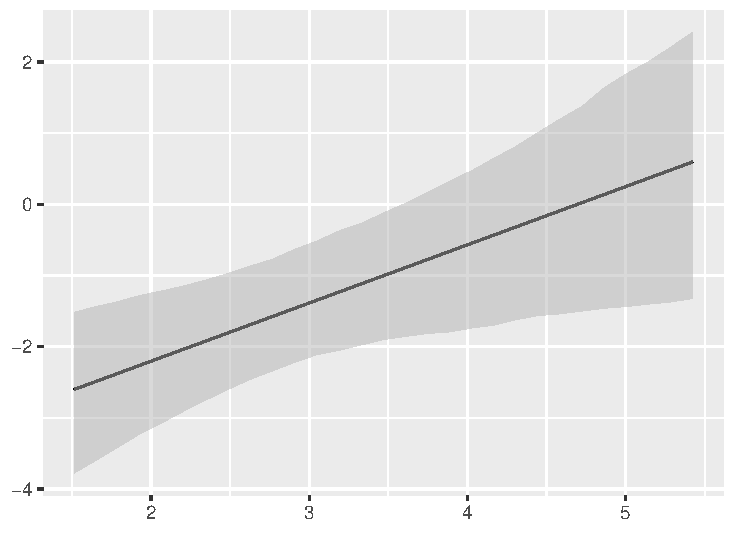
\includegraphics{Interplot-Plot-the-Effects-of-Variables-in-Interaction-Terms_files/figure-pdf/unnamed-chunk-3-1.pdf}

}

\end{figure}

The plot clearly shows that with increasing automobile weight (along the
x axis), the magnitude of the coefficient of the number of cylinders on
the mileage also increases (along the y axis).

Similarly, to show how the number of cylinders affects the coefficient
of automobile weight on mileage, one only needs to switch \texttt{var1}
and \texttt{var2}:

\begin{verbatim}
interplot(m = m_cyl, var1 = "wt", var2 = "cyl")
\end{verbatim}

\begin{figure}[H]

{\centering 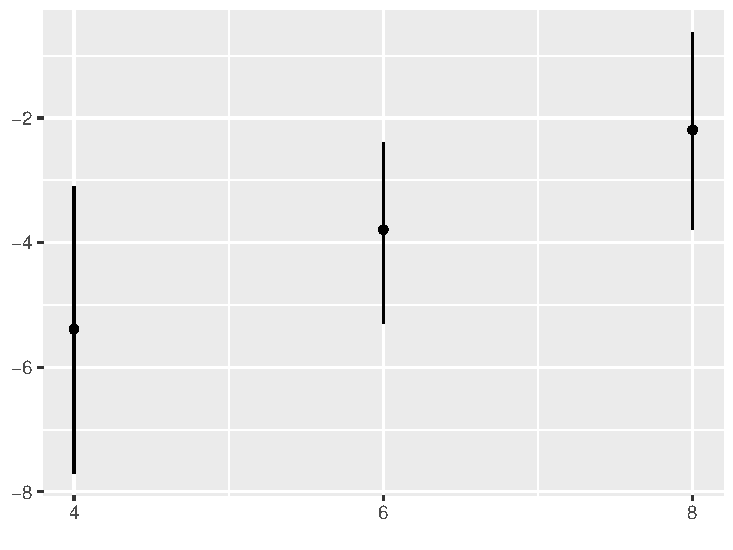
\includegraphics{Interplot-Plot-the-Effects-of-Variables-in-Interaction-Terms_files/figure-pdf/unnamed-chunk-4-1.pdf}

}

\end{figure}

Users can adjust the CI level by setting the \texttt{ci} option. The
default value is 95\% CIs. The following example resets the the CIs to
90\%.

\begin{verbatim}
interplot(m = m_cyl, var1 = "wt", var2 = "cyl", ci = .9, point = T)
\end{verbatim}

\begin{figure}[H]

{\centering 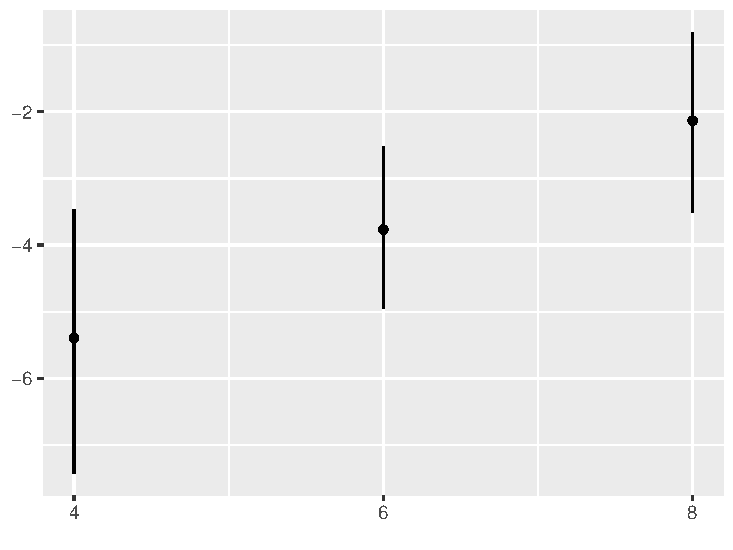
\includegraphics{Interplot-Plot-the-Effects-of-Variables-in-Interaction-Terms_files/figure-pdf/unnamed-chunk-5-1.pdf}

}

\end{figure}

The format of the plot also changes when \texttt{wt} is \texttt{var1}
and \texttt{cyl} is \texttt{var2}. This is because \texttt{cyl} is not a
continuous variable but a categorical one with just three values: 4, 6,
and 8. \texttt{interplot} automatically detects the number of values
taken on by \texttt{var2} and chooses the appropriate plot format. If
there are fewer than 10 values, the function will produce a
``dot-and-whisker'' plot; otherwise, by default, it will generate a
``line-and-ribbon'' plot. Users may override this default by setting the
argument \texttt{point} to \texttt{TRUE}.

\begin{verbatim}
interplot(m = m_cyl, var1 = "cyl", var2 = "wt", point = T) +

  # changing the angle of x labels for a clearer vision
  theme(axis.text.x  = element_text(angle=90))
\end{verbatim}

\begin{figure}[H]

{\centering 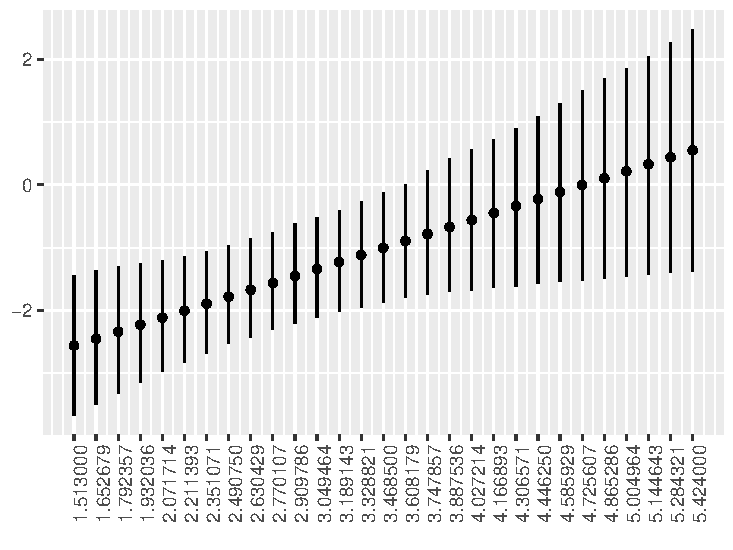
\includegraphics{Interplot-Plot-the-Effects-of-Variables-in-Interaction-Terms_files/figure-pdf/unnamed-chunk-6-1.pdf}

}

\end{figure}

\hypertarget{sec-change-the-appearance-of-the-plot}{%
\subsection{Change the Appearance of the
Plot}\label{sec-change-the-appearance-of-the-plot}}

Plots generated by \texttt{interplot} are, by design, very basic. They
are, however, \texttt{ggplot} objects and so may be easily modified
further.

\begin{verbatim}
interplot(m = m_cyl, var1 = "cyl", var2 = "wt") + 

  # Add labels for X and Y axes
    xlab("Automobile Weight (thousands lbs)") +
    ylab("Estimated Coefficient for\nNumber of Cylinders") +
    
  # Change the background
    theme_bw() +
    
  # Add the title
    ggtitle("Estimated Coefficient of Engine Cylinders \non Mileage by Automobile Weight") +
    theme(plot.title = element_text(face="bold")) +
    
  # Add a horizontal line at y = 0
    geom_hline(yintercept = 0, linetype = "dashed")
\end{verbatim}

\begin{figure}[H]

{\centering 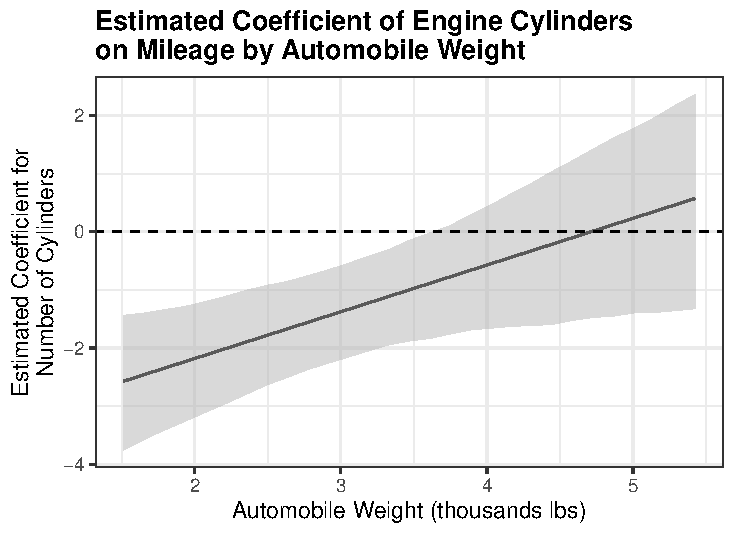
\includegraphics{Interplot-Plot-the-Effects-of-Variables-in-Interaction-Terms_files/figure-pdf/unnamed-chunk-7-1.pdf}

}

\end{figure}

For the default settings of the whisker or ribbon, the users can also
use arguments, such as \texttt{ercolor} and \texttt{esize} to modify.
More arguments can be found in the \texttt{?interplot} file.

\begin{verbatim}
interplot(m = m_cyl, var1 = "wt", var2 = "cyl", ercolor = "blue", esize = 1.5) +
  geom_point(size = 2, color = "red")
\end{verbatim}

\begin{figure}[H]

{\centering 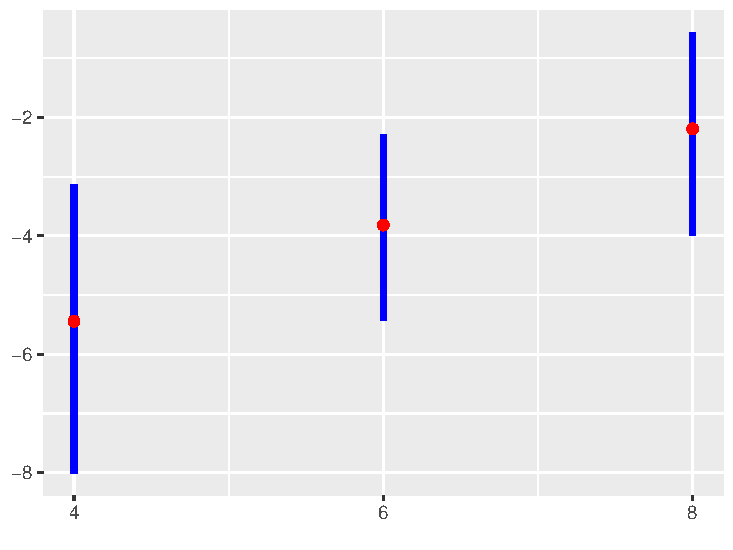
\includegraphics{Interplot-Plot-the-Effects-of-Variables-in-Interaction-Terms_files/figure-pdf/unnamed-chunk-8-1.pdf}

}

\end{figure}

\hypertarget{sec-plot-the-effect-of-a-variable-with-a-quadratic-term}{%
\subsection{Plot the Effect of a Variable with a Quadratic
Term}\label{sec-plot-the-effect-of-a-variable-with-a-quadratic-term}}

The simplest type of interaction is quadratic term, which can be
regarded as a variable interact with itself. \texttt{interplot} can
visualize this case when the variable names of \texttt{var1} and
\texttt{var2} are the same.

\begin{verbatim}
m_wt <- lm(mpg ~ wt + I(wt^2), data = mtcars)

interplot(m = m_wt, var1 = "wt", var2 = "wt")
\end{verbatim}

\begin{figure}[H]

{\centering 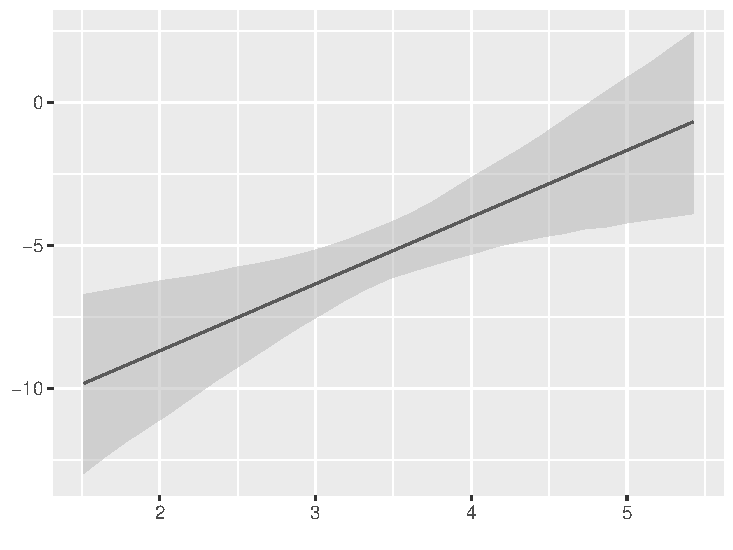
\includegraphics{Interplot-Plot-the-Effects-of-Variables-in-Interaction-Terms_files/figure-pdf/unnamed-chunk-9-1.pdf}

}

\end{figure}

\hypertarget{plot-interactions-with-a-factor-term}{%
\subsection{Plot Interactions with a Factor
Term}\label{plot-interactions-with-a-factor-term}}

When either the conditioned or the conditioning base term of an
interaction is a factor,~\texttt{interplot}~creates a facet in which the
conditional effect under each category of the factor is visualized in a
separate panel.

\begin{verbatim}
mtcars$gear <- factor(mtcars$gear)
m_gear <- lm(mpg ~ gear * wt, data = mtcars)

interplot(m = m_gear, var1 = "wt", var2 = "gear")
\end{verbatim}

\begin{figure}[H]

{\centering 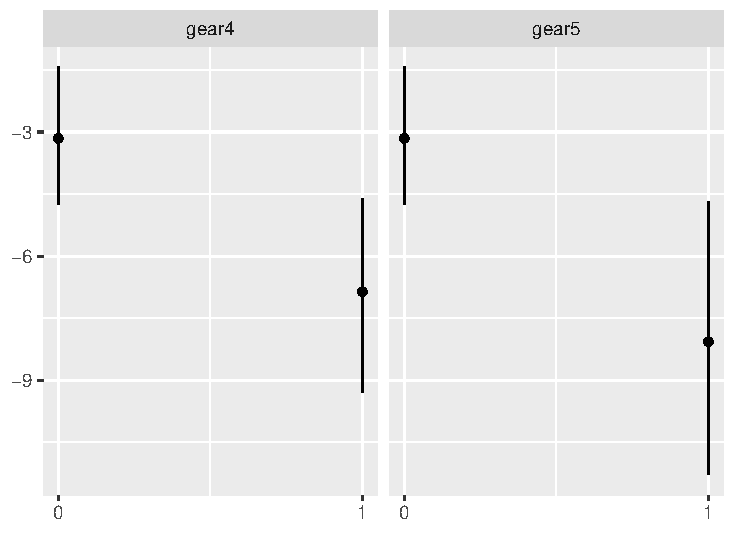
\includegraphics{Interplot-Plot-the-Effects-of-Variables-in-Interaction-Terms_files/figure-pdf/unnamed-chunk-10-1.pdf}

}

\end{figure}

To edit the facet labels, use the \texttt{facet\_labs} argument to
specify a character vector of the desired labels:

\begin{verbatim}
interplot(m = m_gear, var1 = "wt", var2 = "gear", facet_labs = c("4-speed", "5-speed"))
\end{verbatim}

\begin{figure}[H]

{\centering 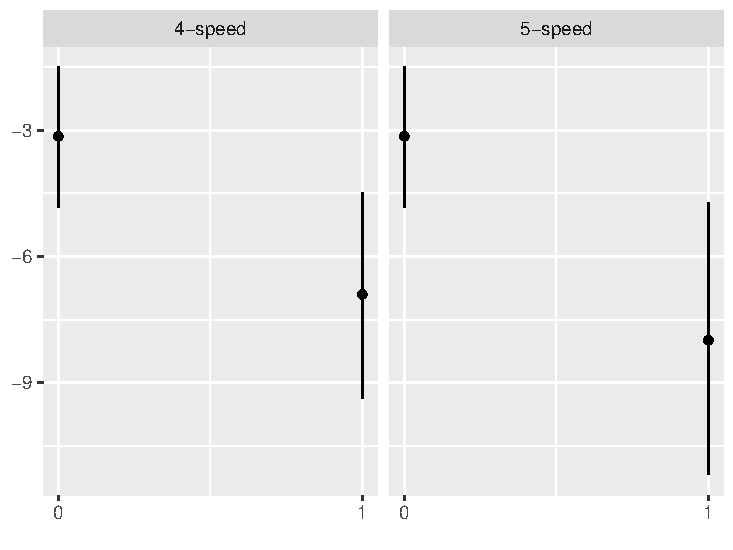
\includegraphics{Interplot-Plot-the-Effects-of-Variables-in-Interaction-Terms_files/figure-pdf/unnamed-chunk-11-1.pdf}

}

\end{figure}

\hypertarget{sec-include-the-distribution-of-the-conditioning-variable}{%
\subsection{Include the Distribution of the Conditioning
Variable}\label{sec-include-the-distribution-of-the-conditioning-variable}}

\citep{BerryGolderMilton2012} points out that, when a variable's
conditional effect reaches statistical significance over only part of
the range of the conditioning variable, it can be helpful to the
evaluation of the substantive significance of the conditional effect to
know the distribution of the conditioning variable. For this purpose,
\texttt{interplot} has the \texttt{hist} argument for users to choose to
superimpose a histogram at the bottom of the conditional effect plot.

\begin{verbatim}
interplot(m = m_cyl, var1 = "cyl", var2 = "wt", hist = TRUE) +
    geom_hline(yintercept = 0, linetype = "dashed")
\end{verbatim}

\begin{figure}[H]

{\centering 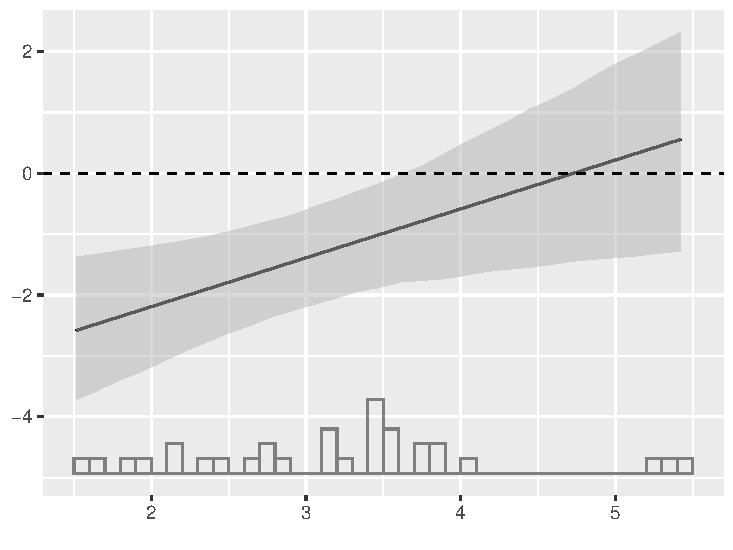
\includegraphics{Interplot-Plot-the-Effects-of-Variables-in-Interaction-Terms_files/figure-pdf/unnamed-chunk-12-1.pdf}

}

\end{figure}

Our implementation of this option was inspired by the excellent work
of~Hainmueller, Mummolo, and Xu (2016). A tip is that when presenting
the histogram, some default setting would not be directly modified by
the build-in arguments or the \texttt{geom} functions. Instead, one can
change these settings by the \texttt{aes} function---as illustrated by
the following example.

\begin{verbatim}
interplot(m = m_cyl, var1 = "cyl", var2 = "wt", hist = TRUE) +

  aes(color = "pink") + theme(legend.position="none") +  # geom_line(color = "pink") + 
  
  geom_hline(yintercept = 0, linetype = "dashed")
\end{verbatim}

\begin{figure}[H]

{\centering 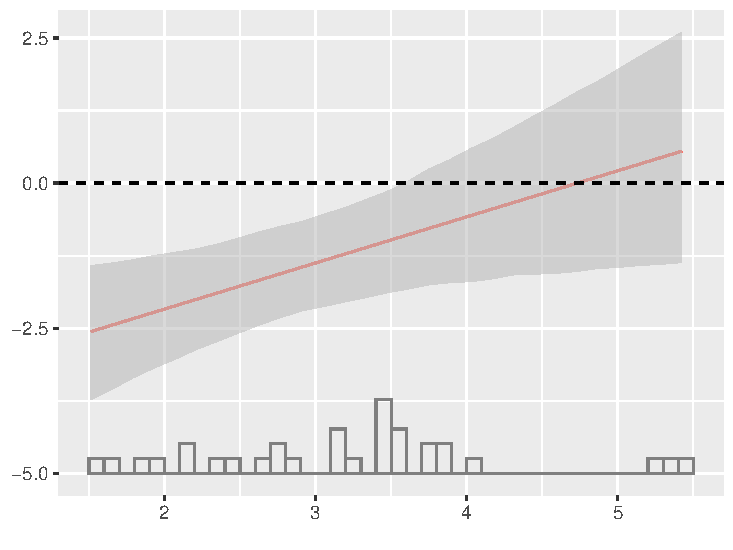
\includegraphics{Interplot-Plot-the-Effects-of-Variables-in-Interaction-Terms_files/figure-pdf/unnamed-chunk-13-1.pdf}

}

\end{figure}

\hypertarget{sec-advanced-use-and-customization}{%
\section{Advanced Use and
Customization}\label{sec-advanced-use-and-customization}}

\hypertarget{sec-statistical-test-of-the-conditional-effect}{%
\subsection{Statistical Test of the Conditional
Effect}\label{sec-statistical-test-of-the-conditional-effect}}

\texttt{interplot} visualizes the conditional effect based on simulated
marginal effects. The simulation provides a probabilistic distribution
of moderation effect of the conditioning variable (\texttt{var2}) at
every preset values (including the minimum and maximum values) of the
conditioned variable (\texttt{var1}), denoted as E\textsubscript{min}
and E\textsubscript{max}. This output allows the function to further
examine the conditional effect statistically in two ways. One is to
examine if the distribution of (E\textsubscript{max} -
E\textsubscript{min}) covers zero. The other is to directly compare
E\textsubscript{min} and E\textsubscript{max} through statistical tools
for distributional comparisons. Users can choose either method by
setting the argument \texttt{stats\_cp} to ``ci'' or ``ks.''

\begin{itemize}
\item
  ``ci'' provides the confidence interval of the difference of
  (E\textsubscript{max} - E\textsubscript{min}). An interval including 0
  suggests no statistical difference before and after the conditional
  effect is applied, and vise versa.
\item
  ``ks'' presents the result of a two-sample Kolmogorov-Smirnov test of
  the simulated distributions of E\textsubscript{min} and
  E\textsubscript{max}. The output includes a D statistics and a p-value
  of the null hypothesis that the two distributions come from the same
  distribution at the 0.05 level.
\end{itemize}

\begin{verbatim}
set.seed(313)

interplot(m = m_cyl, var1 = "cyl", var2 = "wt", stats_cp = "ci")
\end{verbatim}

\begin{figure}[H]

{\centering 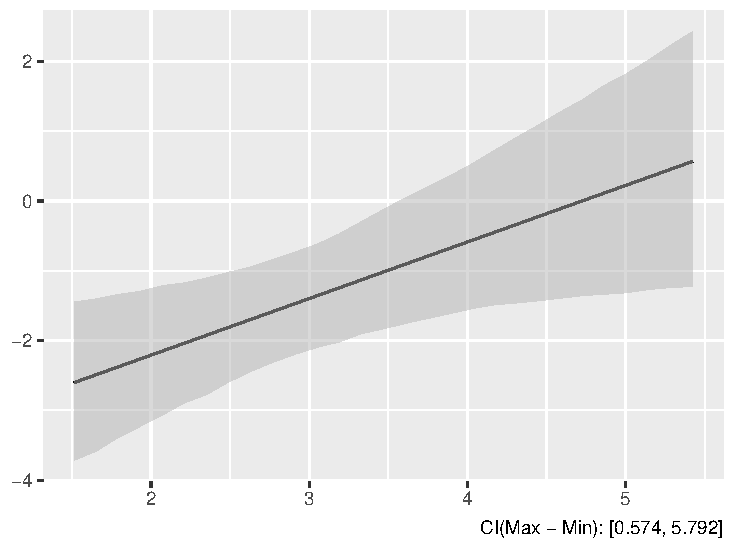
\includegraphics{Interplot-Plot-the-Effects-of-Variables-in-Interaction-Terms_files/figure-pdf/unnamed-chunk-14-1.pdf}

}

\end{figure}

\begin{verbatim}
interplot(m = m_cyl, var1 = "cyl", var2 = "wt", stats_cp = "ks")
\end{verbatim}

\begin{figure}[H]

{\centering 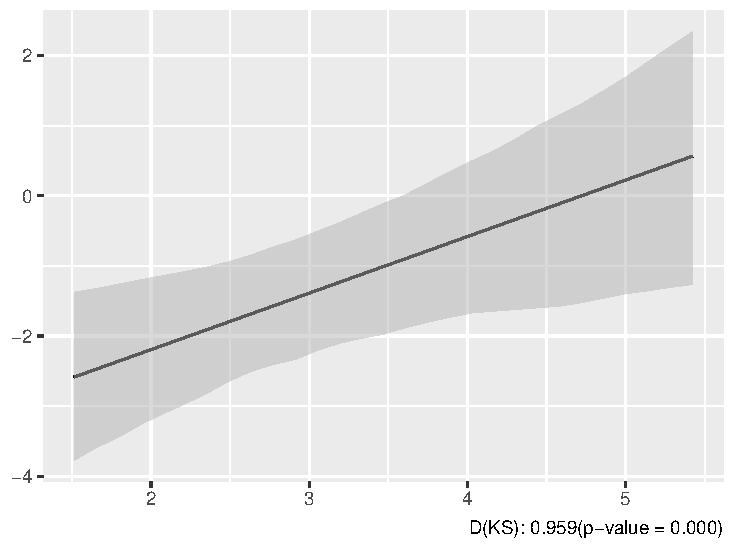
\includegraphics{Interplot-Plot-the-Effects-of-Variables-in-Interaction-Terms_files/figure-pdf/unnamed-chunk-15-1.pdf}

}

\end{figure}

since the statistical results are presented as a \texttt{ggplot}
caption, one cannot using \texttt{+\ lab(caption\ =\ ...)} to specify it
as for a regular \texttt{ggplot} object. Instead, users can modify the
plot's caption by specify the argument \texttt{txt\_caption} of the
\texttt{dwplot} function.

\begin{verbatim}
set.seed(313)

interplot(m = m_cyl, var1 = "cyl", var2 = "wt", stats_cp = "ci", txt_caption = "\n Source: Motor Trend Car Road Tests 1973.")
\end{verbatim}

\begin{figure}[H]

{\centering 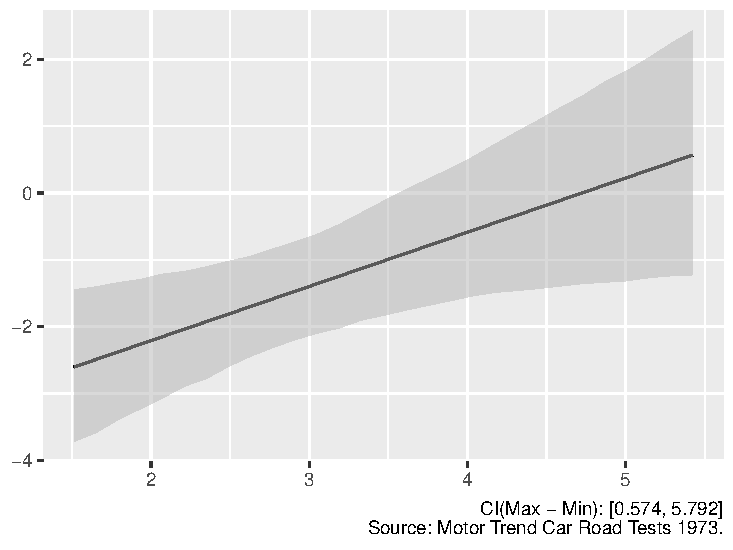
\includegraphics{Interplot-Plot-the-Effects-of-Variables-in-Interaction-Terms_files/figure-pdf/unnamed-chunk-16-1.pdf}

}

\end{figure}

\hypertarget{sec-adjust-the-overconfidence-in-confidence-interval-estimations}{%
\subsection{Adjust the Overconfidence in Confidence Interval
Estimations}\label{sec-adjust-the-overconfidence-in-confidence-interval-estimations}}

\citep{BerryDeMerittEsarey2016} emphasized the importance to estimate
the uncertainty in studying conditional effects. The most common way to
do that is to follow the straightforward method of
\citep{BramborClarkGolder2006}. Nevertheless, \citep{EsareySumner2018}
pointed out that this method might cause a ``multiple comparison
problem'' and result over- or underconfidence of the confidential
intervals. For the overconfidence cases, they recommended to adjust the
CIs with a critical t-statistics following the Benjamini1995 procedure.

\texttt{interplot} incorporates this recommendation with an argument
\texttt{adjCI}. If it is set \texttt{TRUE}, the function will calculate
the critical t-statistics to limit the false discovery rate and adjust
the estimation of confidence intervals. In the following example, the
left panel presents the conditional effect plot with CIs estimated based
on the \citep{BramborClarkGolder2006} method, and the right panel
presents results with adjusted CIs. Although the adjustment does not
change the substantial conclusion, we can see the adjusted CIs cover
more area both in the middle and at the extreme values of x.

\begin{verbatim}
stdCI_plot <- interplot(m = m_wt, var1 = "wt", var2 = "wt", adjCI = FALSE) +
ggtitle("Marginal Effects with Standard CIs")

adjCI_plot <- interplot(m = m_wt, var1 = "wt", var2 = "wt", adjCI = TRUE) +
ggtitle("Marginal Effects with Adjusted CIs")

library(gridExtra)
\end{verbatim}

\begin{verbatim}
Warning: package 'gridExtra' was built under R version 4.3.1
\end{verbatim}

\begin{verbatim}
grid.arrange(stdCI_plot, adjCI_plot, ncol = 2)
\end{verbatim}

\begin{figure}[H]

{\centering 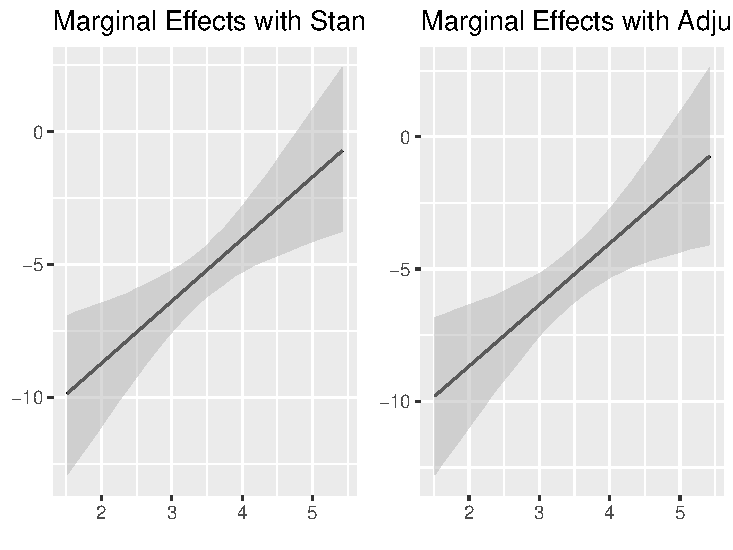
\includegraphics{Interplot-Plot-the-Effects-of-Variables-in-Interaction-Terms_files/figure-pdf/unnamed-chunk-17-1.pdf}

}

\end{figure}

\hypertarget{plot-conditional-predicted-probability}{%
\subsection{Plot Conditional Predicted
Probability}\label{plot-conditional-predicted-probability}}

\citep{HanmerOzanKalkan2013} point out (also in the associated
\href{https://ajps.org/2014/11/13/translating-statistical-results-into-meaningful-quantities-methods/}{post}
in the AJPS website) that it is important to translate statistical
results into meaningful quantities. The task not only pushes researchers
to interpret the results in a real-life manner---which may lead to
substantively different conclusions---but also provides convenience for
a far broader scope of readers (e.g., policy makers, governmental
officials, stakeholders, etc.) to understand the implications of the
study and their importance.

To accomplish this task requires researchers to go beyond estimating the
effect for the ``average case,'' but focuses more on the values or
intervals that are illustratively important and meaningful. This could
be a time-consuming job, though, especially when researchers work on
models with limited dependent variables. \texttt{interplot} provides a
convenient way to achieve the task. When researchers are dealing with
general linear flat or multilevel models, they have the choice to set
the argument \texttt{predPro} to \texttt{TRUE} and give the critical
values they are interested in the argument \texttt{var2\_vals}. Then,
\texttt{interplot} will automatically estimated the conditional effects
of predicted probabilities at these given values of the conditioned
variable. The following example illustrates how it works.

In this example, we are interested how the economic inequality affect
the impact of income on the U.S. citizens' belief in meritocracy, a
critical ideology of the ``American Dream.'' We estimated this
conditional effect based on an interaction model with three years of Pew
surveys (2006, 2007, and 2009), in which the income is the conditioned
variable and economic inequality (county-level Gini
coefficients).\footnote{For the purpose of illustration, we omitted the
  county level variance in this example. One can see more comprehensive
  analyses in \citep{solt2017}.}We first estimate the average
conditional effect for the entire sample and then estimate the
conditional predicted probabilities for citizens with the lowest and
highest levels of income separately. As shown in the following plot, the
average case in the left panel only shows a decreasing conditional
effect, while the predicted probability plot in the right uncovers
conditional effects in opposite directions for the high and low income
individuals.

\begin{verbatim}
pew1.w <- read.csv("pew1_w.csv")


m <- glm(formula=meritocracy~ginicnty+income_i+ginicnty:income_i+income_cnty+black_cnty+
                perc_bush04+pop_cnty+educ_i+age_i+gender_i+unemp_i+union_i+partyid_i+
                ideo_i+attend_i+survid2006+survid2007+survid2009,
              data=pew1.w,family=binomial(link="logit"))
 
              
plot_avg <- interplot(m, var1 = "ginicnty",var2 = "income_i", predPro = FALSE) + 
ggtitle("Average Conditional Effects")


plot_3val <- interplot(m, var1 = "ginicnty",var2 = "income_i", predPro = TRUE, var2_vals = c(min(pew1.w$income_i), max(pew1.w$income_i))) +
ggtitle("Conditional Predicted Probabilities for \nCitizens with Low and High Incomes") +
scale_colour_discrete(guide = guide_legend(title = "Income"), labels = c("Low", "High")) + 
scale_fill_discrete(guide = guide_legend(title = "Income"), labels = c("Low", "High")) +
theme(legend.position = c(0, .8), legend.justification = c(0, .5))
\end{verbatim}

\begin{verbatim}
Warning: `funs()` was deprecated in dplyr 0.8.0.
i Please use a list of either functions or lambdas:

# Simple named list: list(mean = mean, median = median)

# Auto named with `tibble::lst()`: tibble::lst(mean, median)

# Using lambdas list(~ mean(., trim = .2), ~ median(., na.rm = TRUE))
i The deprecated feature was likely used in the interplot package.
  Please report the issue at <https://github.com/sammo3182/interplot/issues>.
\end{verbatim}

\begin{verbatim}
grid.arrange(plot_avg, plot_3val, ncol = 2)
\end{verbatim}

\begin{figure}[H]

{\centering 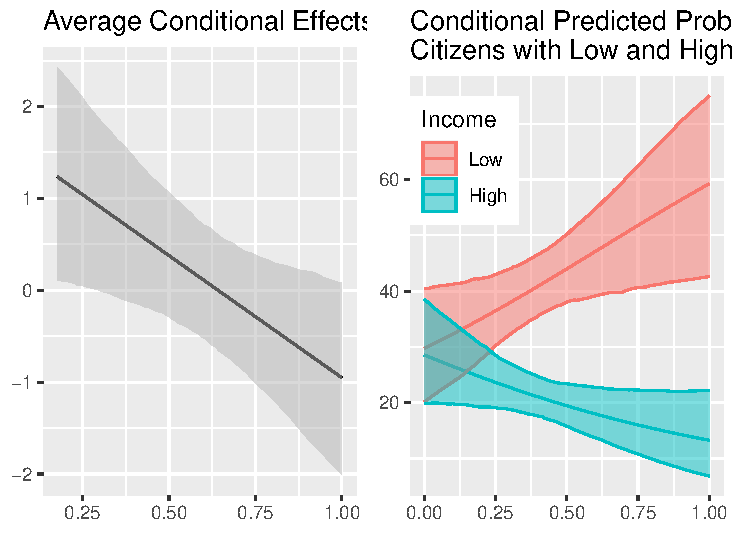
\includegraphics{Interplot-Plot-the-Effects-of-Variables-in-Interaction-Terms_files/figure-pdf/unnamed-chunk-18-1.pdf}

}

\end{figure}

\hypertarget{sec-plot-conditional-effects-without-a-model}{%
\subsection{Plot Conditional Effects Without a
Model}\label{sec-plot-conditional-effects-without-a-model}}

In some cases, one may analyze some complicated or self-made regression
functions which are not supported by the current version of
\texttt{interplot}. For such models, as long as the user has a dataset
loading the simulated results of the interaction effects, she can still
use \texttt{interplot} to visualize it. The dataset needs four columns
the scale of the conditioning variable (\texttt{fake}), the simulated
interactive effect at each break of the conditioning variable
(\texttt{coef1}), and the simulated lower bound and upper bound of the
confidence interval (\texttt{lb}, and \texttt{ub}). The column names
should be exactly the ones shown in the above parentheses. Here is an
example with some arbitrary artificial data:

\begin{verbatim}
# Create a fake dataset of conditional effects
fake <- rnorm(100, 0, 1)
coef1 <- fake * sample(.5:2.5, 100, replace = T)
lb <- coef1 - .5
ub <- coef1 + .5

df_fake <- data.frame(cbind(fake, coef1, lb, ub))


# Use interplot directly with the dataset
interplot(df_fake)
\end{verbatim}

\begin{figure}[H]

{\centering 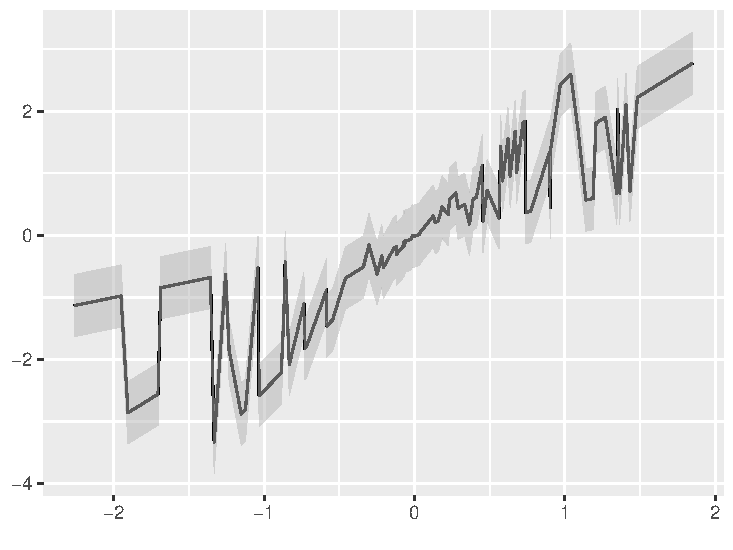
\includegraphics{Interplot-Plot-the-Effects-of-Variables-in-Interaction-Terms_files/figure-pdf/unnamed-chunk-19-1.pdf}

}

\end{figure}

If one also has the data of the \texttt{var2}, she can also draw a
histogram under it by the argument \texttt{var\_dt}.

\begin{verbatim}
var2_fake <- fake

# Set `hist` to TRUE is required to superimpose a histogram.
interplot(df_fake, hist = TRUE, var2_dt = var2_fake)
\end{verbatim}

\begin{figure}[H]

{\centering 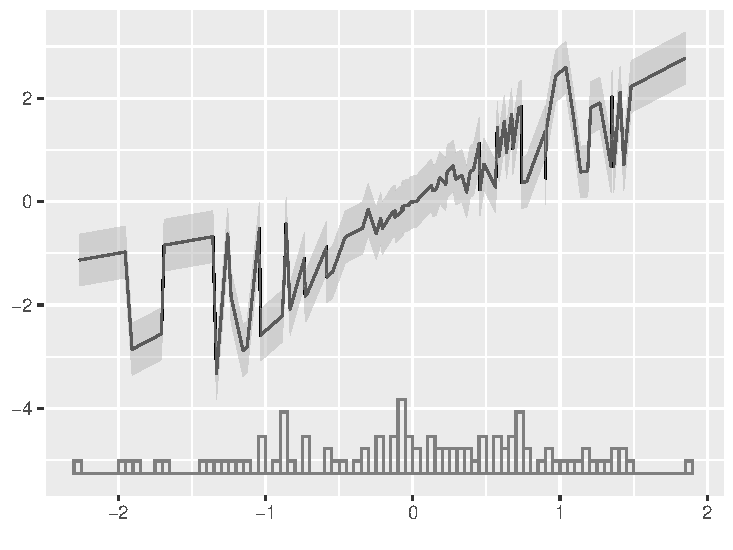
\includegraphics{Interplot-Plot-the-Effects-of-Variables-in-Interaction-Terms_files/figure-pdf/unnamed-chunk-20-1.pdf}

}

\end{figure}

\hypertarget{sec-conclusion}{%
\section{Conclusion}\label{sec-conclusion}}

The \texttt{interplot} package provides a flexible and convenient way to
visualize conditional coefficients of variables in multiplicative
interaction terms. This vignette offers an overview of its use and
features. We encourage users to consult the help files for more details.

The development of the package is ongoing, and future research promises
a compatible tool for more types of regressions and more functions.
Please contact us with any questions, bug reports, and comments.

\hypertarget{sec-references}{%
\section*{References}\label{sec-references}}
\addcontentsline{toc}{section}{References}

\renewcommand{\bibsection}{}
\bibliography{jss_interplot.bib}




\end{document}
